\documentclass[12pt,a4paper]{article}
\usepackage[utf8]{inputenc}
\usepackage[export]{adjustbox}
\usepackage{amsmath}
\usepackage{amsfonts}
\usepackage{amssymb}
\usepackage{xcolor}
\usepackage{graphicx}
\usepackage{subcaption}
\usepackage[left=2cm,right=2cm,top=2cm,bottom=2cm]{geometry}

\newcommand{\frc}[2]{\raisebox{2pt}{$#1$}\big/\raisebox{-3pt}{$#2$}}

\author{Maksym Polovyi}
\title{Colloid MC}
\begin{document}
\section{Model}

We consider colloidal particles with a permanent dipole moment $\mu \hat{m}$, where $\hat{m}$ is is a unitary vector with the direction of the dipole moment. While considering a three-dimensional system, we constrain particle positions to a one-dimensional line, i.e., particles are confined to positions along the z axis. However, particles can explore the full three dimensional orientation space. \textcolor{red}{um, I thougth that $z$ axis is a definition in itself? Just in case, how do I define it?}

The particle-particle interaction consists of two contributions: a dipole-dipole interaction and a short-range repulsion.

The energy of dipole-dipole interaction is given by

\label{eq_dipole_dipole_interaction}
\begin{equation}
E_{12} = - \frac{\mu_1 \mu_2}{\Delta r^3}[3 (\hat{m}_1 \cdot \hat{r}_{12})(\hat{m}_2 \cdot \hat{r}_{12}) - (\hat{m}_1 \cdot \hat{m}_2)]
\end{equation}
where $\mu_1 \hat{m}_1$ and $\mu_2 \hat{m}_2$ are dipole moments of interacting particles, $\vec{r}_{12}$ is the direction vector which connects particle centres whereas $\Delta r$ stands for the distance between particle centers.

By constraining particles in 1D tube we effectively enforce $\vec{r}_{12}$ to be co-aligned with $z$ axis. Defining energy in the units of particle dipole moment and assuming that all particles have the same dipole moment, (\ref{eq_dipole_dipole_interaction}) can be simplified in the following way:

\label{eq_dipole_dipole_1D}
\begin{equation}
E_{12}^{attr} = - \frac{1}{\Delta z^3} [3 \cos \theta_1 \cos \theta_2 - (\hat{m}_1 \cdot \hat{•}{m}_2)]
\end{equation}
where $\theta_1$ and $\theta_2$ are the angles between $z$ axis and dipole moments of the first and second particle respectfully, and $\Delta z = |z_2 - z_1|$, where $z_1$ and $z_2$ are displacements of particle centers along $z$ axis. Because of three-dimensionality of our model, we can't simplify the last term, which accounts for relative orientation of the particles.

The repulsive part is described by Yukawa potential
\label{eq_yukawa_interaction}
\begin{equation}
E_{12}^{rep} = \frac{A \exp(-k \Delta z)}{\Delta z}
\end{equation}
Summarizing all of the above, the particle-particle interaction potential is presented in the following form:
\label{eq_full_particle_particle_interraction}
\begin{equation}
E_{12} = \left\{ \frac{A \exp(-k \Delta z)}{\Delta z} -  \frac{1}{\Delta z^3} [3 \cos \theta_1 \cos \theta_2 - (\hat{m}_1 \cdot \hat{m}_2)]\right\}
\end{equation}
where $A$ and $k$ -- parameters which governs repulsion hardness and coupling energy. Figure \ref{fig:interaction_energy} show examples of $E_{12}$ for different parameters.

\begin{figure}[h]
\begin{subfigure}{\textwidth}
\begin{subfigure}{.5\textwidth}
	\centering
	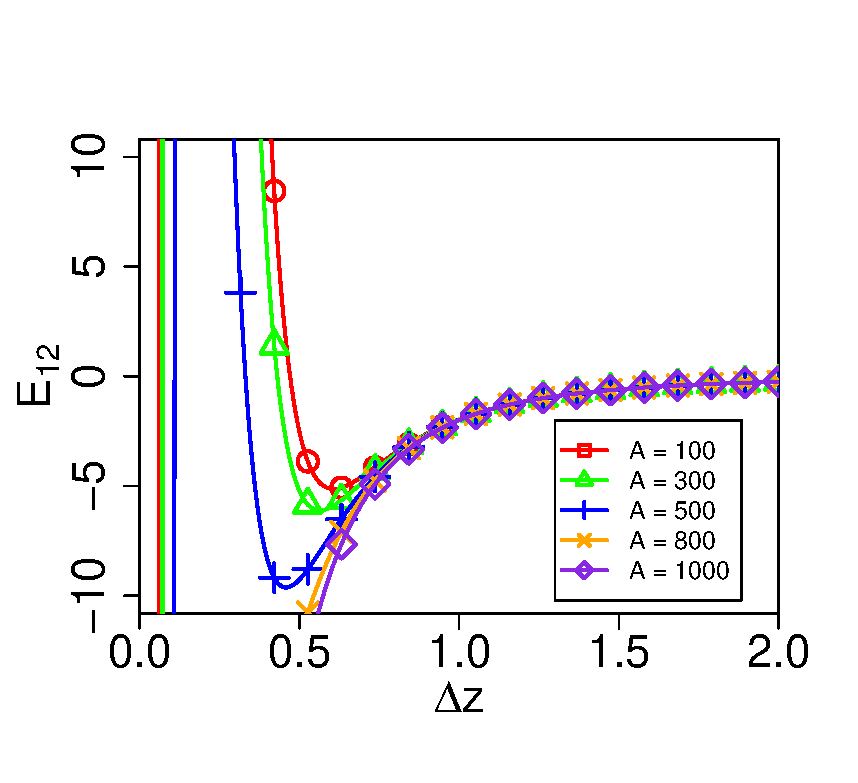
\includegraphics[width=.9\textwidth]{k=10}
\end{subfigure}
\begin{subfigure}{.5\textwidth}
	\centering
	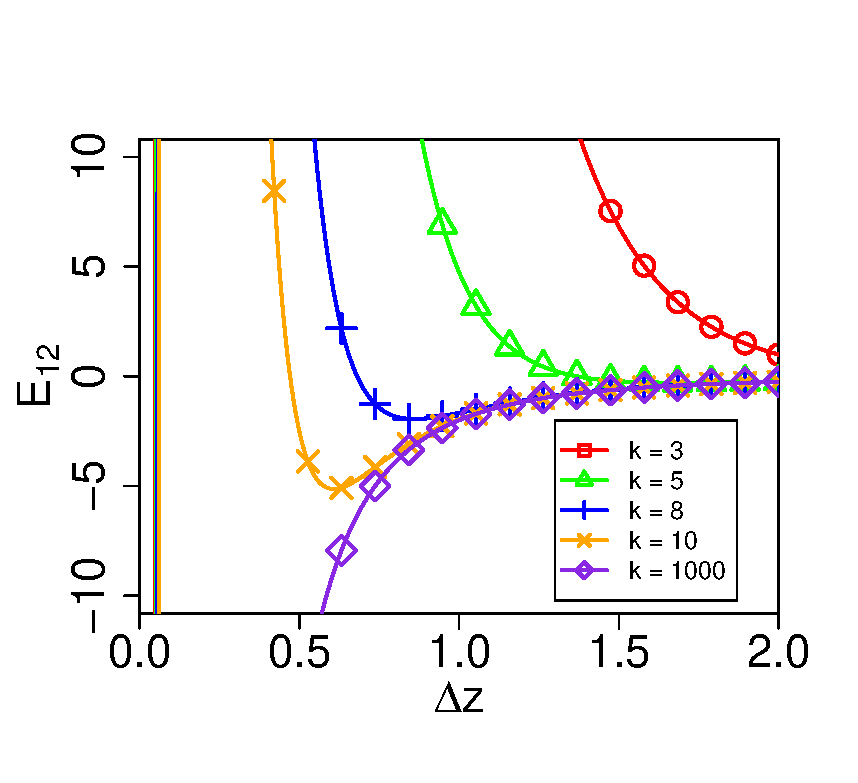
\includegraphics[width=.9\textwidth]{A=1000}
\end{subfigure}
	\captionsetup{justification=centering, width=0.7\textwidth, singlelinecheck=false}
	\caption{Particles dipole moments are both co-aligned with $z$ axis}
    \label{fig:interaction_energy_coaligned}
\end{subfigure}

\begin{subfigure}{\textwidth}
\begin{subfigure}{.5\textwidth}
	\centering
	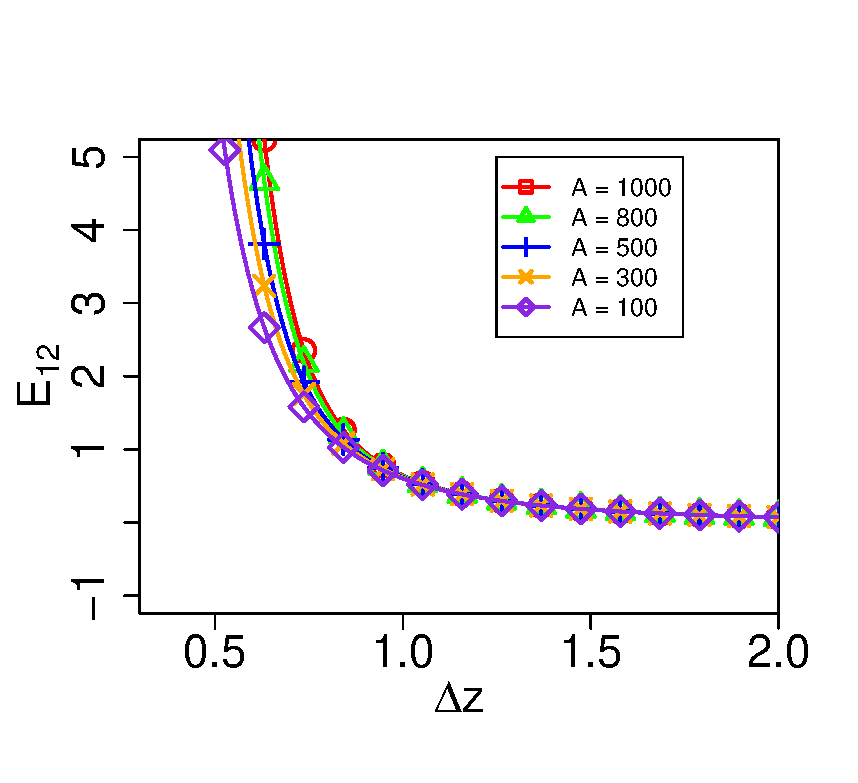
\includegraphics[width=.9\textwidth]{k=10_perp}
\end{subfigure}
\begin{subfigure}{.5\textwidth}
	\centering
	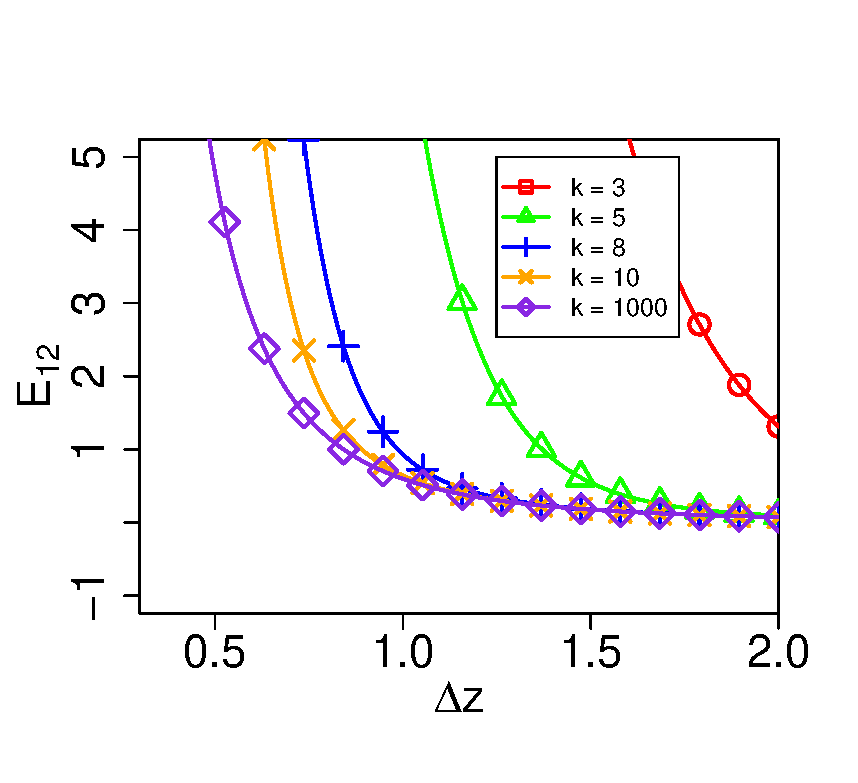
\includegraphics[width=.9\textwidth]{A=1000_perp}
\end{subfigure}
	\captionsetup{justification=centering, width=0.7\textwidth, singlelinecheck=false}
	\caption{First particle dipole moment is co-aligned and second particle dipole moment is perpendicular to $z$ axis}
    \label{fig:interaction_energy_counteraligned}
\end{subfigure}
\captionsetup{justification=centering, width=0.8\textwidth}
\caption{Interaction energy as function of distance between centres of two interacting particles for co-aligned (\ref{fig:interaction_energy_coaligned}) and perpendicular (\ref{fig:interaction_energy_counteraligned}) orientation of the particles}
\label{fig:interaction_energy}
\end{figure}

For the case when particles dipole moments are perpendicular to each other the interaction is purely repulsive. However, as we can see on the Figure \ref{fig:interaction_energy_coaligned}, for low values of $A$, combined with high values of $k$, we can observe purely attractive interaction. Since this behaviour is physically impossible, we assumed $A = 1000$ and $k = 10$.

%\begin{figure}[h]
%    \centering
%	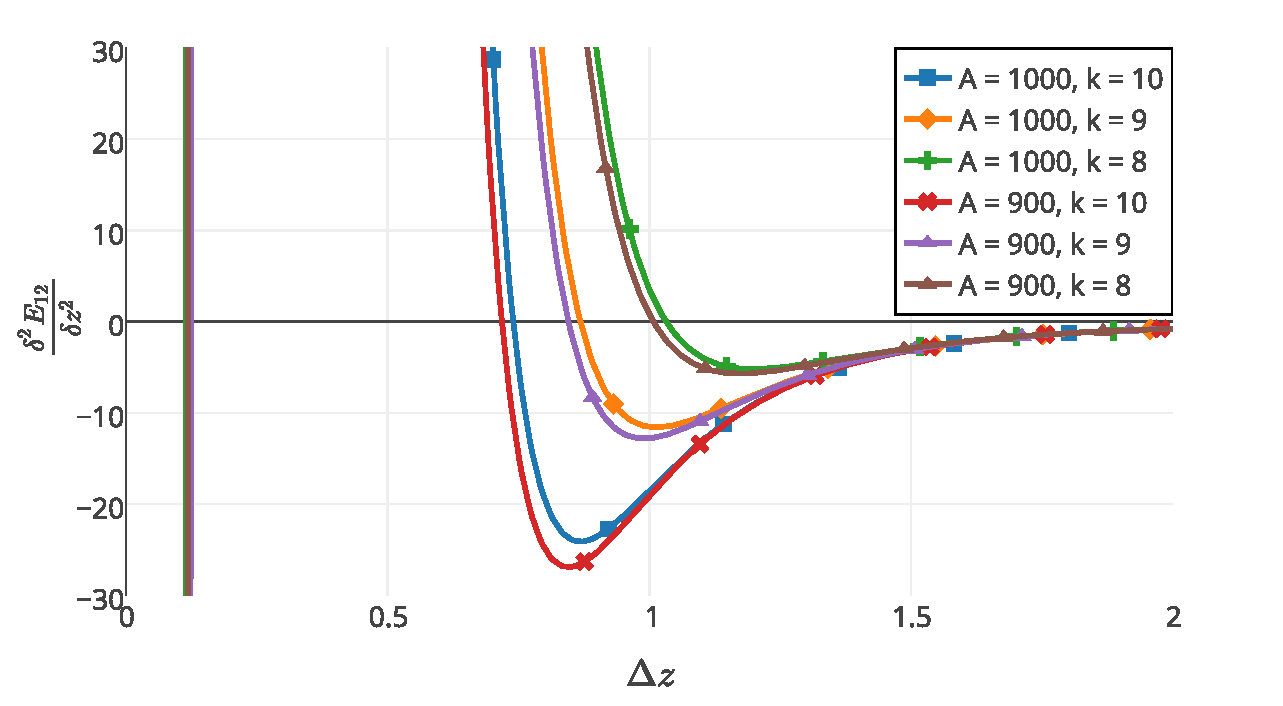
\includegraphics[width=.6\textwidth]{Energy_deriv2_r_difAK}
%	\captionsetup{justification=centering, width=0.8\textwidth}
%	\caption{Second derivative of interaction energy as function of distance between centres of two co-aligned particles ($\theta_1 = \theta_2 = 0$)}
%	\label{fig:energy_second_derivative}
%\end{figure}

\section{Monte Carlo Simulations}

At first we concentrate on the equilibrium state of the system. For that we implement a common MC algorithm in a following way.

Every test step we choose a particle at random. Than we subject the particle to the \emph{test move} and \emph{test rotation}.

Test move is a particle displacement ($z_{t+1} = z_t + \Delta z$) \textcolor{red}{$\Delta z$ here means different than in formulas 1-4, should I invent new name here?}, where $\Delta z$ is a random value evenly distributed in $[+\delta, -\delta]$, with $\delta = 0.5 (r_{min} - r_0)$. 

Test rotation consists of generating new orientation of the particle at random, evenly distributed over all orientation space.

After move and rotation test step is evaluated with standard Metropolis acceptance criteria.

For the sake of simplicity we restrict interactions to the immediate neighbours (particle $i$ interacts only with $i-1$ and $i+1$ particles) 

On each end of the system we implement continuous border conditions.

\section{Production runs and results}

In our simulations we considered a density $\rho = 0.5$.  

Defining $\rho = \frac{N d}{L}$ where $N$ --- number of particles and $d$ --- particle diameter, we immediately obtain the simulation system size $L = \frac{Nd}{\rho}$.

As diameter of a particle we have taken the position of the minimum of (\ref{eq_full_particle_particle_interraction}), obtained when particles dipole moments are co-aligned (see Figure \ref{fig:interaction_energy_coaligned}). \textcolor{red}{diameter calculated by newton method + checked - any displacement leads to function increase. Should I explain it? Not analytically because I'm better with computer than math. And I calculate it every run to get system size}

Important question is the length (number of test steps taken) of simulations (\textcolor{red}{Here will be order parameter as function of MonteCarlo sweeps picture? or how should I explain why I'm doing $10^8$ sweeps?}).

We concentrate on the following quantities.

Order parameter $S$ defined in standard way:
\begin{equation}
S = \frac{3 \overline{\cos^2 \theta} - 1}{2}
\end{equation}
where $\theta$ it the angle between particle direction and spatial axis, while horizontal bar denotes mean over all particles.

Orientation correlation as function of distance between particles:
\begin{equation}
\langle\cos \theta_1 \cos \theta_2\rangle \propto |z_2 - z_1|
\end{equation}

And particle chains length probability distribution \textcolor{red}{How to call it??}. One can think of different ways to define it, but the simplest is the following: two particles considered to be "chained" if 
\begin{equation}
\begin{cases}
	|z_1 - z_2| &\leq d\\
	\cos \theta_1 \cdot \cos \theta_2 &\geq 0
\end{cases}
\end{equation}

Second check enforces bonded particles to have same sign of projection of the dipole moment vector on the spatial axis. As we will show in the \textcolor{red}{Results} section, this is unnecessary, since on the equilibrium chained (by distance) particles tend to have the same orientation.

\cite{Camp2000}

\bibliographystyle{plain}
\bibliography{Bibliography}
\end{document}